\section{From Correlation to Causality}

Having established correlations between \Length, \rr, \failedstep, and correctness, we now ask whether these correlations hold causally. We design two experiments: first, test-time selection using each metric (Section \ref{sec:test-time-select}); second, controlled CoT editing targeting \fsf (Section \ref{sec:edit-cot}).

\subsection{Test-time selection}\label{sec:test-time-select}

{We now use test-time selection as a causal probe. Beyond correlations, we ask whether a metric leads to higher accuracy when it serves as the rule that picks the best final answer. For each question, we hold the candidate set fixed (same model and decoding) and intervene on the selection policy: we re-rank candidates by the metric and take the top-1. This intervention changes only the distribution of the final selected output. A strong metric should preferentially select correct solutions, yielding the highest pass@1 under this intervention.}

\paragraph{Setup} We evaluate on AIME 2025 (30 problems), which is widely regarded as contamination-free math dataset for recent LRMs, and on the full GPQA-Diamond set. For each problem and model, we sample 64 independent generations. For a given metric, we rank the 64 candidates and compute pass@1 from the top-1. We compare four selectors: (i) \fsf (lower is better), (ii) \Length (shorter is better), (iii) \rr (lower is better, opposite for Claude 3.7), and (iv) random selection. Since pass@1 can be noisy in this regime, we estimate uncertainty via bootstrap: for each model–problem, we draw 200 replicates by resampling the 64 candidates with replacement, re-rank by each selector, record top-1 accuracy, aggregate over problems, and report the mean and standard deviation across replicates. Results are shown in Figure~\ref{fig:pass_1_aime}. 

\paragraph{Results} We observe that \fsf is the strongest selector across models and datasets. On AIME 2025, choosing the single best candidate by FSF yields gains of roughly 5–13\% over the random baseline. \fsf delivers consistent and significant improvements for all models. \rr and \Length also improve accuracy for most models, with the exception of \Length on GPT oss 120B. On GPQA-Diamond, \fsf again produces significant gains for every model. These interventions provide \emph{causal evidence} for all metrics, with the strongest and the most consistent effect for \fsf. {Notably, \fsf is estimated by Claude 3.7, the weakest model on math reasoning in Figure \ref{fig:pass_1_aime}, without access to the ground truth answers, yet it still yields consistent accuracy gains for all models. In this design, we do not rely on a strong judge, we do not provide ground truth answers, and we only ask the model to extract the graph (not to label correctness), which minimizes the risk of knowledge leakage. When Claude 3.7 both generates and estimates \fsf and then selects by it (self generate, self estimate, self select), accuracy improves by up to 12\% for math.}


% FSF also outperforms using Claude directly as a judge, considering the fact that FSF does not involve any correctness judgement about the solution, but rather structural extractions. It suggests that the structural signal extracted from the CoT is more informative and inherent than a black-box verdict. FSF could select all the correct generations with top@8. By contrast, Length is only weakly predictive at small k and drops below random at k=16.

\begin{figure}[tb]
    \centering
    \vspace{-10pt}
    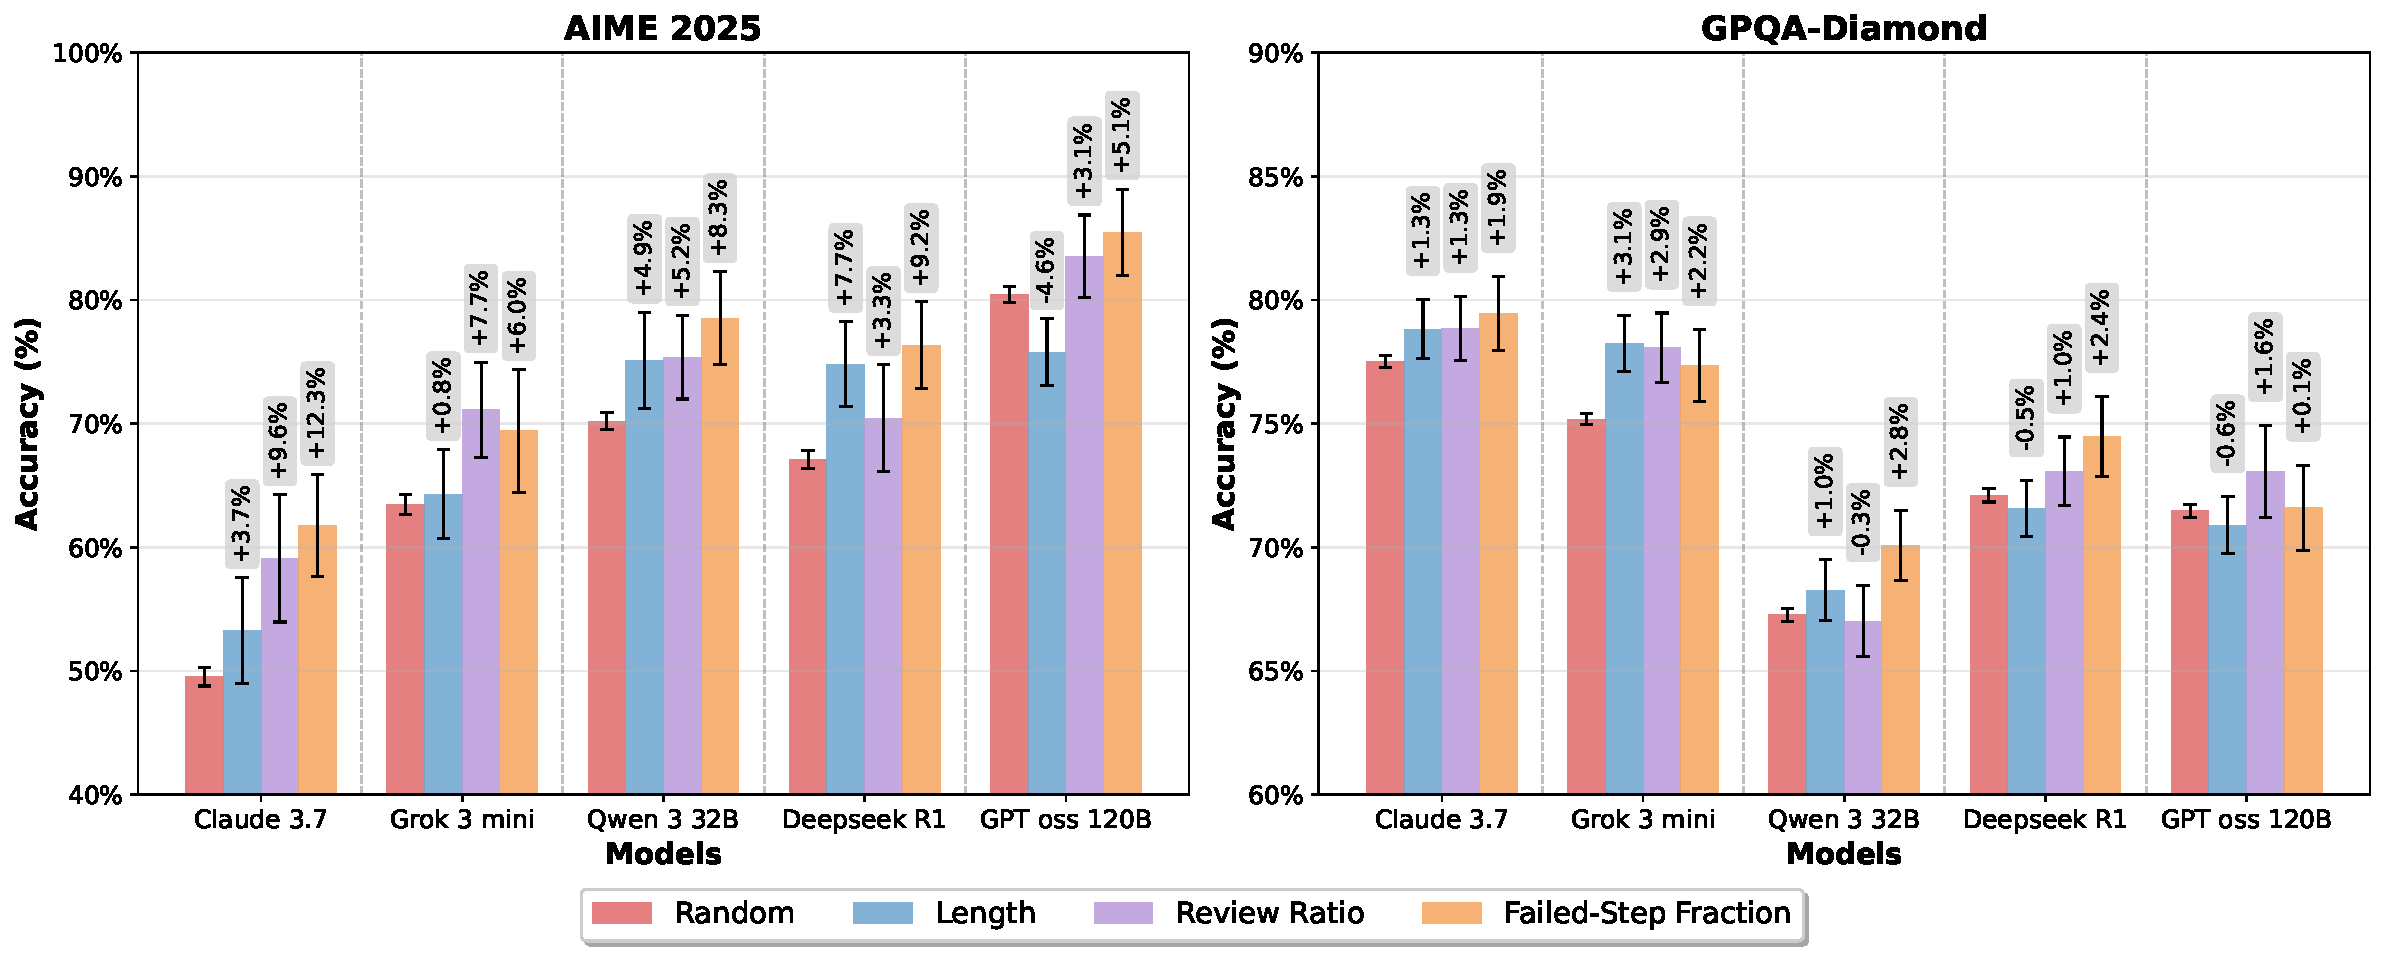
\includegraphics[width=\linewidth]{final_figs/test_time_selection.pdf}
    % \includegraphics[width=0.8\linewidth]{fig_tmp/gqpa_pass_1.png}
    \caption{Pass@1 with test-time selection by \length, \rr, and \fsf. Error bars show bootstrap standard deviations. \fsf generally achieves the largest gains, supporting its role as a causal lever.}
    \label{fig:pass_1_aime}
\end{figure}

\begin{tcolorbox}[colback=metablue!7]
In conclusion, \failedstep is the strongest metric that holds causally.
\end{tcolorbox}


\subsection{Modifying the CoT}\label{sec:edit-cot}
In this section we further investigate:
 Why does higher \failedstep harm performance? Within the correlation test in Section \ref{sec:graph-result}, we further examine whether the depth of the first failed-step correlates with correctness. The result is included in Figure \ref{fig:motivation_all_correlation} as 'First Failed Step Depth'. We find little to no correlation across all models. This suggests that it is the presence and extent of failed attempts, rather than when they occur, that harms performance. This observation motivates the following controlled edit: would removing failed exploration improve the accuracy? 
 
To do so, we must first identify where each failed exploration starts. Specifically, when extracting the reasoning graph with Claude 3.7, we also ask it to identify where a failed branch begins (full prompt in Appendix \ref{append-intervention}). We then remove that branch, from its start through the failed attempt steps, and evaluate how its removal changes the accuracy of the partial CoT. We apply this procedure to 80 incorrect HARP traces generated by Deepseek R1 and 160 incorrect traces generated by GPT oss 120B. We compare three variants, each evaluated at both the first and the last failed branch (six settings total): (1) the original reasoning prefix containing the failed branch, with all subsequent steps truncated; (2) the reduced reasoning prefix that includes only the steps up to the failed branch; and (3) the initial prefix plus a concise summary of the failed branch. For each partial CoT in each setting, we perform eight continuation generations to reliably assess accuracy, without a token-budget limit. We perform 11,520 continuation generations in total. Figure~\ref{fig:cot_continue} illustrates our CoT-editing procedure and the continuation generation used to probe accuracy.


\begin{wrapfigure}{r}{0.5\textwidth}
\begin{minipage}{\linewidth}
  \centering
  \vspace{-10pt}
  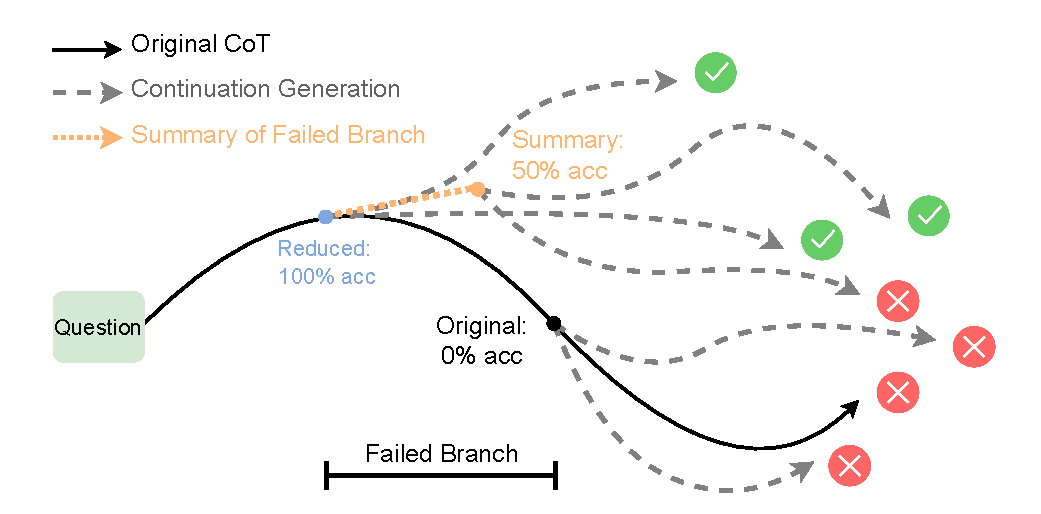
\includegraphics[width=\linewidth]{final_figs/cot_continue.pdf}
  \caption{Visualization of the continuation generation setup. For incorrect CoTs, we either remove the failed branch or append a brief summary, then evaluate accuracy by continuing from the partial CoT (gray dashed arrows). Table \ref{tab:intervention} are reported for three setups: \emph{reduced} (failed branch removed), \emph{original} (failed branch retained), and \emph{summary}.}
  \label{fig:cot_continue}
  \vspace{-20pt}
\end{minipage}
\end{wrapfigure}


Table \ref{tab:intervention} reports the results. For both models, removing the failed branch, at either the first or last failed point, substantially increases the accuracy (the probability that the existing partial CoT reaches the correct answer), by roughly 8–14\%. This indicates that the models are capable of producing a successful generation, but the presence of a failed branch markedly lowers that probability. Providing a short summary of the failed branch also improves accuracy, though not as much as removing it entirely. Overall, these results suggest that long failed branches bias subsequent exploration even after backtracking; current models do not fully “unsee” past mistakes. Overall, our findings support \emph{quality-aware test-time scaling}: prefer structure-aware selection \citep{yao2023tree, bi2024forest} and context management with targeted branch pruning/summarization \citep{snell2024scaling, hao2025rl, liao2025fractured} over indiscriminately generating longer CoTs.

% \todo{Make a teaser to explain the setup.}


% The generation length in the test are:

% For Deepseek R1: 8527; 22404; 16641; 31656; all std: 0.0136; 0.0166; 0.0138; 0.0098; 0.0136; 0.0137;

% For GPT oss 120B: 6955; 12749; 13255; 22012; Avg zero acc: 0.452. All std: 0.0085; 0.0095; 0.0090; 0.0071; 0.0085; 0.0089.


% \begin{table}[htb]
%     \centering
%     \begin{tabular}{c|l|ccc}
% \hline
% Model & & Original & Reduced & Reduced with Summary \\
% \hline
% \multirow{2}{*}{Deepseek R1} & First Failed Branch & 0.2089 & 0.2942 & 0.2814 \\
%  & Last Failed Branch  & 0.0972 & 0.2375 & 0.2257 \\
% \hline
% \multirow{2}{*}{GPT oss 120B} & First Failed Branch & 0.2805 & 0.3641 & 0.2951 \\
%  & Last Failed Branch  & 0.1650 & 0.2733 & 0.2522 \\
% \hline
% \end{tabular}
%     \caption{We edit the CoT by deleting failed branches or replacing them with summaries, and measure the effect on accuracy using 8 continuation generations per CoT.}
%     \label{tab:intervention}
% \end{table}

\begin{table}[tb]
\small
    \centering
    \caption{Accuracy reported as mean $\pm$ standard deviation (in \%). We edit the CoT by deleting failed branches or replacing them with summaries, and measure the effect on accuracy using 8 continuation generations per CoT. Edit performed on a subset of incorrect CoTs from HARP. Removing the failed branch significantly improve the accuracy.}
    \label{tab:intervention}
    \begin{tabular}{c|l|ccc}
\hline
Model & & Original & Reduced & Reduced with Summary \\
\hline
\multirow{2}{*}{Deepseek R1} & First Failed Branch & 20.89\% ($\pm$1.36\%) & 29.42\% ($\pm$1.66\%) & 28.14\% ($\pm$1.38\%) \\
 & Last Failed Branch  & 9.72\% ($\pm$0.98\%) & 23.75\% ($\pm$1.36\%) & 22.57\% ($\pm$1.37\%) \\
\hline
\multirow{2}{*}{GPT oss 120B} & First Failed Branch & 28.05\% ($\pm$0.85\%) & 36.41\% ($\pm$0.95\%) & 29.51\% ($\pm$0.90\%) \\
 & Last Failed Branch  & 16.50\% ($\pm$0.71\%) & 27.33\% ($\pm$0.85\%) & 25.22\% ($\pm$0.89\%) \\
\hline
\end{tabular}
\end{table}

\begin{tcolorbox}[colback=metablue!7]
In conclusion, failed branches harm performance by biasing subsequent exploration; removing them improves accuracy.
\end{tcolorbox}



% \subsection{Instrument Variable}



% \section{What does it mean to test-time compute?}

% Does the result conflict with the common test-time scaling curve we seen? Not really. When limiting the reasoning length, we see similar test-time scaling curves when changing the budget. A concurrent paper \citep{wu2025s} also points out that the test-time scaling curve mainly stems from limiting the length, instead of increasing the length. 

% We have the result where we truncate the reasoning to see the test-time scaling.

% \concern{We observe that the model perform better when backtrack less. Is it purely a test-time effect coming from sampling? Does it mean that the model is not able to reliably backtrack, that the prior attempts bias the continue generation?}

% \concern{We have recent papers arguing backtracking is important in training. How does our result connect with training?}

% Why would more Failed-Step Fraction hurt the reasoning? I have validated that the extracted steps are indeed backtracking, and these backtracking are benefits for the model. 



% We present the correlation results on HARP in Figure \ref{fig:correlation_motivation_1}

% \begin{figure}[tb]
%     \centering
%     \includegraphics[width=\linewidth]{fig_tmp/pass_1/correlation_motivation_1.png}
%     % \includegraphics[width=\linewidth]{fig_tmp/pass_1/correlation_motivation_2.png}
%     \caption{Correlation results for Review Centroid, Switch Count, and motivation level. HARP dataset.}
%     \label{fig:correlation_motivation_1}
% \end{figure}

% \begin{figure}[tb]
%     \centering
%     \includegraphics[width=0.45\linewidth]{fig_tmp/pass_1/correlation_depth_1.png}
%     % \includegraphics[width=0.45\linewidth]{fig_tmp/pass_1/correlation_depth_2.png}
%     \caption{Correlation results for reasoning graph depth. HARP dataset.}
%     \label{fig:correlation_depth_1}
% \end{figure}


